%%%%%%%%%%%%%%%%%%%%%%%%%%%%%%%%%%%%%%%%%
% Proceedings of the National Academy of Sciences (PNAS)
% LaTeX Template
% Version 1.0 (19/5/13)
%
% This template has been downloaded from:
% http://www.LaTeXTemplates.com
%
% Original author:
% The PNAStwo class was created and is owned by PNAS:
% http://www.pnas.org/site/authors/LaTex.xhtml
% This template has been modified from the blank PNAS template to include
% examples of how to insert content and drastically change commenting. The
% structural integrity is maintained as in the original blank template.
%
% Original header:
%% PNAStmpl.tex
%% Template file to use for PNAS articles prepared in LaTeX
%% Version: Apr 14, 2008
%
%%%%%%%%%%%%%%%%%%%%%%%%%%%%%%%%%%%%%%%%%

%----------------------------------------------------------------------------------------
%	PACKAGES AND OTHER DOCUMENT CONFIGURATIONS
%----------------------------------------------------------------------------------------

%------------------------------------------------
% BASIC CLASS FILE
%------------------------------------------------

%% PNAStwo for two column articles is called by default.
%% Uncomment PNASone for single column articles. One column class
%% and style files are available upon request from pnas@nas.edu.

%\documentclass{pnasone}
\documentclass{pnastwo}

%------------------------------------------------
% POSITION OF TEXT
%------------------------------------------------

%% Changing position of text on physical page:
%% Since not all printers position
%% the printed page in the same place on the physical page,
%% you can change the position yourself here, if you need to:

% \advance\voffset -.5in % Minus dimension will raise the printed page on the 
                         %  physical page; positive dimension will lower it.

%% You may set the dimension to the size that you need.

%------------------------------------------------
% GRAPHICS STYLE FILE
%------------------------------------------------

%% Requires graphics style file (graphicx.sty), used for inserting
%% .eps/image files into LaTeX articles.
%% Note that inclusion of .eps files is for your reference only;
%% when submitting to PNAS please submit figures separately.

%% Type into the square brackets the name of the driver program 
%% that you are using. If you don't know, try dvips, which is the
%% most common PC driver, or textures for the Mac. These are the options:

% [dvips], [xdvi], [dvipdf], [dvipdfm], [dvipdfmx], [pdftex], [dvipsone],
% [dviwindo], [emtex], [dviwin], [pctexps], [pctexwin], [pctexhp], [pctex32],
% [truetex], [tcidvi], [vtex], [oztex], [textures], [xetex]

\usepackage{graphicx}

%------------------------------------------------
% OPTIONAL POSTSCRIPT FONT FILES
%------------------------------------------------

%% PostScript font files: You may need to edit the PNASoneF.sty
%% or PNAStwoF.sty file to make the font names match those on your system. 
%% Alternatively, you can leave the font style file commands commented out
%% and typeset your article using the default Computer Modern 
%% fonts (recommended). If accepted, your article will be typeset
%% at PNAS using PostScript fonts.

% Choose PNASoneF for one column; PNAStwoF for two column:
%\usepackage{PNASoneF}
%\usepackage{PNAStwoF}

%------------------------------------------------
% ADDITIONAL OPTIONAL STYLE FILES
%------------------------------------------------

%% The AMS math files are commonly used to gain access to useful features
%% like extended math fonts and math commands.

\usepackage{amssymb,amsfonts,amsmath}

%------------------------------------------------
% OPTIONAL MACRO FILES
%------------------------------------------------

%% Insert self-defined macros here.
%% \newcommand definitions are recommended; \def definitions are supported

%\newcommand{\mfrac}[2]{\frac{\displaystyle #1}{\displaystyle #2}}
%\def\s{\sigma}

%------------------------------------------------
% DO NOT EDIT THIS SECTION
%------------------------------------------------

%% For PNAS Only:
\contributor{Submitted to Proceedings of the National Academy of Sciences of the United States of America}
\url{www.pnas.org/cgi/doi/10.1073/pnas.0709640104}
\copyrightyear{2008}
\issuedate{Issue Date}
\volume{Volume}
\issuenumber{Issue Number}

%----------------------------------------------------------------------------------------

\begin{document}

%----------------------------------------------------------------------------------------
%	TITLE AND AUTHORS
%----------------------------------------------------------------------------------------

\title{The Effects of Intraspecific Genetic Variation on the Dynamics of Predator-Prey Ecological Communities} % For titles, only capitalize the first letter

%------------------------------------------------

%% Enter authors via the \author command.  
%% Use \affil to define affiliations.
%% (Leave no spaces between author name and \affil command)

%% Note that the \thanks{} command has been disabled in favor of
%% a generic, reserved space for PNAS publication footnotes.

%% \author{<author name>
%% \affil{<number>}{<Institution>}} One number for each institution.
%% The same number should be used for authors that
%% are affiliated with the same institution, after the first time
%% only the number is needed, ie, \affil{number}{text}, \affil{number}{}
%% Then, before last author ...
%% \and
%% \author{<author name>
%% \affil{<number>}{}}

%% For example, assuming Garcia and Sonnery are both affiliated with
%% Universidad de Murcia:
%% \author{Roberta Graff\affil{1}{University of Cambridge, Cambridge,
%% United Kingdom},
%% Javier de Ruiz Garcia\affil{2}{Universidad de Murcia, Bioquimica y Biologia
%% Molecular, Murcia, Spain}, \and Franklin Sonnery\affil{2}{}}

\author{Samuel R. Fleischer\affil{1}{California State University, Northridge}
\and
Pablo Chavarria\affil{1}{Califronia State University, Northridge}}

\contributor{PUMP Final Report $\bullet$ May 2015 $\bullet$ Pacific Math Alliance}

%----------------------------------------------------------------------------------------

\maketitle % The \maketitle command is necessary to build the title page

\begin{article}

%----------------------------------------------------------------------------------------
%	ABSTRACT, KEYWORDS AND ABBREVIATIONS
%----------------------------------------------------------------------------------------

\begin{abstract}
Recent ecological models have incorporated evolutionary variables in order to further understand predator/prey and competitive dynamics.  General classifications of possible dynamics exist, but no previous model has provided enough flexibility to generate all dynamics.  We propose a coevolutionary ditrophic model and provide realistic ecologic parameters that produce all dynamics.
\end{abstract}

%------------------------------------------------

% \keywords{Keyword1 | Keyword2 | Keyword3} % When adding keywords, separate each term with a straight line: |

%------------------------------------------------

%% Optional for entering abbreviations, separate the abbreviation from
%% its definition with a comma, separate each pair with a semicolon:
%% for example:
%% \abbreviations{SAM, self-assembled monolayer; OTS,
%% octadecyltrichlorosilane}

% \abbreviations{}

%----------------------------------------------------------------------------------------
%	PUBLICATION CONTENT
%----------------------------------------------------------------------------------------

%% The first letter of the article should be drop cap: \dropcap{} e.g.,
%\dropcap{I}n this article we study the evolution of ''almost-sharp'' fronts

\section{Introduction}

\dropcap{N}atural populations differ in size, morphology, physiology, and behavior.  This genetic variation is a central and organizing theme of evolutionary biology \cite{Schreiber_2011}.

%------------------------------------------------

\section{Model and Methods}

We consider the ditrophic dynamics of $v$ predator populations with densities $M_i = M_i(t)$, consuming $u$ prey populations with densities $N_j = N_j(t)$, respectively ($i = 1, \dots, v$, and $j = 1, \dots, u$).  Ecological parameters will be defined as functions of predator phenotypic values, $m_i$, and prey phenotypic values, $n_j$, of quantitative traits.  Predator traits are normally distributed with mean $\overline{m_i} = \overline{m_i}(t)$ and constant variances $\sigma_i^2$, and prey traits are normally distributed with mean $\overline{n_j} = \overline{n_j}(t)$ and constant variances $\beta_j^2$, i.e., their distributions are given by
\begin{equation}
\label{pred_dists}
p(m_i, \overline{m_i}) = \frac{1}{\sqrt{2\pi\sigma_i^2}}\exp\left[-\frac{(m_i - \overline{m_i})^2}{2\sigma_i^2}\right]
\end{equation}
\begin{equation}
\label{prey_dists}
p(n_j, \overline{n_j}) = \frac{1}{\sqrt{2\pi\beta_j^2}}\exp\left[-\frac{(n_j - \overline{n_j})^2}{2\beta_j^2}\right]
\end{equation}
These variances have genetic and environmental components:
\begin{equation}
\label{pred_variance}
\sigma_i^2 = \sigma_{Gi}^2 + \sigma_{Ei}^2
\end{equation}
\begin{equation}
\label{prey_variance}
\beta_i^2 = \beta_{Gi}^2 + \beta_{Ei}^2
\end{equation}
Assuming predator $i$ has a linear functional response with attack rate $a_{ij} = a_{ij}(m_i, n_j)$, converts consumed prey $j$ into offspring with efficiencies $e_{ij} = e_{ij}(m_i, n_j)$, and experiences a per-capita mortality rate $d_i(m_i)$, then the fitness of a predator with phenotype $m_i$ is
\begin{equation}
	\label{predator_fitness}
	\begin{aligned}
		W_i(N_1, \dots, N_u, &M_i, n_1, \dots, n_v, m_i) \\
		&= \sum\limits_{j = 1}^{u}\left[e_{ij}(m_i, n_j)a_{ij}(m_i, n_j)N_i\right] - d_i(m_i)
	\end{aligned}
\end{equation}
and the mean fitness of the predator population is
\begin{equation}
	\label{avg_predator_fitness}
	\begin{aligned}
		\overline{W_i}&(N_1, \dots, N_u, M_i, \overline{n_1}, \dots, \overline{n_v}, \overline{m_i}) \\
		&= \int\limits_{\mathbb{R}^{u+1}}^{}W_ip(m_i, \overline{m_i})\prod\limits_{j = 1}^{u}p(n_j, \overline{n_j})dm_i\prod\limits_{j = 1}^{u}dn_j
	\end{aligned}
\end{equation}
In the absence of any predators, each prey species experiences logistic-type growth with growth rates $r_j = r_j(n_j)$ and carrying capacities $K_j = K_j(n_j)$.  Under these assumptions, the fitness of a prey individual with phenotype $n_j$ is
\begin{equation}
	\label{prey_fitness}
	\begin{aligned}
		Y_j(&N_j, M_1, \dots, M_v, n_j, m_1, \dots, m_v) \\
		&= r_j(n_j)\left(1 - \frac{N_j}{K_j(n_j)}\right) - \sum\limits_{i = 1}^{v}\left[a_{ij}(m_i, n_j)M_i\right]
	\end{aligned}
\end{equation}
and the mean fitness of the prey population is
\begin{equation}
	\label{avg_prey_fitness}
	\begin{aligned}
		\overline{Y_j}&(N_j, M_1, \dots, M_v, \overline{n_j}, \overline{m_1}, \dots, \overline{m_v}) \\
		&= \int\limits_{\mathbb{R}^{v+1}}^{}Y_jp(n_j, \overline{n_j})\prod\limits_{i = 1}^{v}p(m_i, \overline{m_i})dn_j\prod\limits_{i = 1}^{v}dm_i
	\end{aligned}
\end{equation}
Thus the complete ditrophic model of $v$ predator species and $u$ prey species is given by
\begin{subequations}
	\label{general_model}
	\begin{align}
		\label{eq:general_model_a}
		\frac{dM_i}{dt} &= M_i\overline{W_i} \\[5px]
		\label{eq:general_model_b}
		\frac{dN_j}{dt} &= N_j\overline{Y_j} \\[5px]
		\label{eq:general_model_c}
		\frac{d\overline{m_i}}{dt} &= \sigma_{Gi}^2\frac{\partial \overline{W_i}}{\partial \overline{m_i}} \\[5px]
		\label{eq:general_model_d} 
		\frac{d\overline{n_j}}{dt} &= \beta_{Gj}^2\frac{\partial \overline{Y_j}}{\partial \overline{n_j}}
	\end{align}
\end{subequations}
Lande derived {\bf [\ref{eq:general_model_c}]} and {\bf [\ref{eq:general_model_d}]} under the assumption that the distribution of phenotypes remains Gaussian.  {\bf [\ref{general_model}]} is a special case of Kindrik and Kondrashov's general model of coevolution \cite{Kindrik_1997}.  The defining feature of our model is the distinction between trophic levels, of which we are assuming there are two.  In the following sections we derive two manifestations of {\bf [\ref{general_model}]} by explicitly defining the parameter functions.

\subsubsection{Model 1}
This first example is a coevolutionary analog of Schreiber, B\"urger, and Bolnick's apparent competition model \cite{Schreiber_2011}.  Assume the prey growth rates and carrying capacities, $r_j$ and $K_j$, and the predator death rates and efficiencies, $d_i$, and $e_{ij}$, are constant, but let an individual predator's attack rate on an individual prey, $a_{ij}(m_i, n_j)$, be maximal at an optimal trait difference, $m_i - n_j = \theta_{ij}$, and decrease away from this optimal trait difference in a Gaussian manner, i.e.,
\begin{equation}
\label{attack_rate}
a_{ij}(m_i, n_j) = \alpha_{ij}\exp{\left[-\frac{((m_i - n_j) - \theta_{ij})^2}{2\tau_{ij}^2}\right]}
\end{equation}
where $\alpha_{ij}$ is the maximal attack and $\tau_{ij}$ determines how steeply the attack rate declines with distance from the optimal trait difference $\theta_{ij}$.  In effect, $\tau_{ij}$ determines how phenotypically specialized predator $i$ must be to use prey $j$.  Under these assumptions, the average attack rate of predator species $i$ on prey species $j$ is
\begin{equation}
	\label{average_attack_rate}
	\begin{aligned}
		\overline{a_{ij}}(\overline{m_i}, \overline{n_j}) &= \int\limits_{\mathbb{R}^2}a_{ij}(m_i, n_j)p(m_i, \overline{m_i})p(n_j, \overline{n_j})dm_idn_j \\
		&= \frac{\alpha_{ij}\tau_{ij}}{\sqrt{A_{ij}}}\exp{\left[-\frac{((m_i - n_j) - \theta_{ij})^2}{2A_{ij}}\right]}
	\end{aligned}
\end{equation}
where $A_{ij} = \tau_{ij}^2 + \sigma_i^2 + \beta_j^2$.  {\bf [\ref{avg_predator_fitness}]} and {\bf [\ref{avg_prey_fitness}]} yield eplicit formulas for $\overline{W_i}$ and $\overline{Y_j}$:
\begin{equation}
	\label{model_1_avg_pred_fitness}
	\overline{W_i} = \sum\limits_{j = 1}^{u}\left[e_{ij}\overline{a_{ij}}(\overline{m_i}, \overline{n_j})N_i\right] - d_i
\end{equation}
\begin{equation}
	\label{model_1_avg_prey_fitness}
	\overline{Y_j} = r_j\left(1 - \frac{N_j}{K_j}\right) - \sum\limits_{i = 1}^{v}\left[\overline{a_{ij}}(\overline{m_i}, \overline{n_j})M_i\right]
\end{equation}
The right-hand sides of {\bf [\ref{eq:general_model_c}]} and {\bf [\ref{eq:general_model_d}]} can also be found:
\begin{equation}
	\label{model_1_pred_fitness_partial}
	\frac{\partial \overline{W_i}}{\partial \overline{m_i}} = \sum\limits_{j = 1}^{u}\left[\frac{e_{ij}N_j(\theta_{ij} - (\overline{m_i} - \overline{n_j}))}{A_{ij}}\overline{a_{ij}}(\overline{m_i}, \overline{n_j})\right]
\end{equation}
\begin{equation}
	\label{model_1_prey_fitness_partial}
	\frac{\partial \overline{Y_j}}{\partial \overline{n_j}} = \sum\limits_{i = 1}^{v}\left[\frac{M_i(\theta_{ij} - (\overline{m_i} - \overline{n_j}))}{A_{ij}}\overline{a_{ij}}(\overline{m_i}, \overline{n_j})\right]
\end{equation}
Thus {\bf [\ref{general_model}]} simplifies:
\begin{subequations}
	\label{model1}
	\begin{align}
		\label{eq:model1_a}
		\frac{dM_i}{dt} &= M_i\left[\sum\limits_{j = 1}^{u}\left[e_{ij}\overline{a_{ij}}(\overline{m_i}, \overline{n_j})N_i\right] - d_i\right] \\[5px]
		\label{eq:model1_b}
		\frac{dN_j}{dt} &= N_j\left[r_j\left(1 - \frac{N_j}{K_j}\right) - \sum\limits_{i = 1}^{v}\left[\overline{a_{ij}}(\overline{m_i}, \overline{n_j})M_i\right]\right] \\[5px]
		\label{eq:model1_c}
		\frac{d\overline{m_i}}{dt} &= \sigma_{Gi}^2\sum\limits_{j = 1}^{u}\left[\frac{e_{ij}N_j(\theta_{ij} - (\overline{m_i} - \overline{n_j}))}{A_{ij}}\overline{a_{ij}}(\overline{m_i}, \overline{n_j})\right] \\[5px]
		\label{eq:model1_d}
		\frac{d\overline{n_j}}{dt} &= \beta_{Gj}^2\sum\limits_{i = 1}^{v}\left[\frac{M_i(\theta_{ij} - (\overline{m_i} - \overline{n_j}))}{A_{ij}}\overline{a_{ij}}(\overline{m_i}, \overline{n_j})\right]
	\end{align}
\end{subequations}
If there is only one predator species and one prey species, then {\bf [\ref{model1}]} simplifies:
\begin{subequations}
	\label{MODEL1}
	\begin{align}
		\label{eq:MODEL1_A}
		\frac{dM}{dt} &= M\left[e\overline{a}(\overline{m}, \overline{n})N - d\right] \\[5px]
		\label{eq:MODEL1_B}
		\frac{dN}{dt} &= N\left[r\left(1 - \frac{N}{K}\right) - \overline{a}(\overline{m}, \overline{n})M\right] \\[5px]
		\label{eq:MODEL1_C}
		\frac{d\overline{m_i}}{dt} &= \sigma_{G}^2\frac{eN(\theta - (\overline{m} - \overline{n}))}{A}\overline{a}(\overline{m}, \overline{n}) \\[5px]
		\label{eq:MODEL1_D}
		\frac{d\overline{n_j}}{dt} &= \beta_{G}^2\frac{M(\theta - (\overline{m} - \overline{n}))}{A}\overline{a}(\overline{m}, \overline{n})
	\end{align}
\end{subequations}

\subsubsection{Model 2}
This second model introduces stabilizing selection to Model 1 by assuming each prey species has an optimal trait value by which growth rate is maximized, and decreases away from the optimal trait value in a Gaussian manner, i.e.
\begin{equation}
	\label{growth_rate}
	r_j(n_j) = \rho_j\exp{\left[-\frac{(n_j - \phi_j)^2}{2\gamma_j^2}\right]}
\end{equation}
where $\rho$ is the maximal growth rate and $\gamma_j$ determines how steeply the growth rate declines with distance from the optimal trait value $\phi_j$.  In effect, $\gamma_j$ determines how far prey $j$ can deviate from its optimal trait value while still maintaining an adequate growth rate.  Under these assumptions, the average growth rate of prey species $j$ is
\begin{equation}
	\label{average_growth_rate}
	\begin{aligned}
		\overline{r_j}(\overline{n_j}) &= \int\limits_{\mathbb{R}}^{}r_j(n_j)p(n_j, \overline{n_j})dn_j \\
		&= \frac{\rho_j\gamma_j}{\sqrt{B_j}}\exp\left[-\frac{(\overline{n_j} - \phi_j)^2}{2B_j}\right]
	\end{aligned}
\end{equation}
where $B_j = \beta_j^2 + \gamma_j^2$.  Since $\overline{W_i}$ is not dependent on $r_j$, {\bf [\ref{model_1_avg_pred_fitness}]} suffices, but since $\overline{Y_j}$ is dependent on $r_j$, it must be recalculated. {\bf [\ref{avg_prey_fitness}]} yields
\begin{equation}
	\label{model_2_avg_prey_fitness}
	\overline{Y_j} = \overline{r_j}(\overline{n_j})\left(1 - \frac{N_j}{K_j}\right) - \sum\limits_{i = 1}^{v}\left[\overline{a_{ij}}(\overline{m_i}, \overline{n_j})M_i\right]
\end{equation}
Since $\overline{W_i}$ did not change from Model 1, {\bf [\ref{eq:model1_c}]} is sufficient for the right hand side of {\bf [\ref{eq:general_model_c}]}.  However, the right hand side of {\bf [\ref{eq:general_model_d}]} must be recalculated.

\begin{equation}
	\label{model_2_prey_fitness_partial}
	\begin{aligned}
		\frac{\partial \overline{Y_j}}{\partial \overline{n_j}} = \overline{r_j}(\overline{n_j})&\left(1 - \frac{N_j}{K_j}\right)\frac{\phi_j - \overline{n_j}}{B_j}\\
		+ &\sum\limits_{i = 1}^{v}\left[\frac{M_i(\theta_{ij} - (\overline{m_i} - \overline{n_j}))}{A_{ij}}\overline{a_{ij}}(\overline{m_i}, \overline{n_j})\right]
	\end{aligned}
\end{equation}
Thus {\bf [\ref{general_model}]} simplifies:
\begin{subequations}
	\label{model2}
	\begin{align}
		\label{eq:model2_a}
		\frac{dM_i}{dt} &= M_i\left[\sum\limits_{j = 1}^{u}\left[e_{ij}\overline{a_{ij}}(\overline{m_i}, \overline{n_j})N_i\right] - d_i\right] \\[5px]
		\label{eq:model2_b}
		\frac{dN_j}{dt} &= N_j\left[\overline{r_j}(\overline{n_j})\left(1 - \frac{N_j}{K_j}\right) - \sum\limits_{i = 1}^{v}\left[\overline{a_{ij}}(\overline{m_i}, \overline{n_j})M_i\right]\right] \\[5px]
		\label{eq:model2_c}
		\frac{d\overline{m_i}}{dt} &= \sigma_{Gi}^2\sum\limits_{j = 1}^{u}\left[\frac{e_{ij}N_j(\theta_{ij} - (\overline{m_i} - \overline{n_j}))}{A_{ij}}\overline{a_{ij}}(\overline{m_i}, \overline{n_j})\right] \\[5px]
		\label{eq:model2_d}
		\begin{split}
			\frac{d\overline{n_j}}{dt} &= \beta_{Gj}^2\Bigg[\overline{r_j}(\overline{n_j})\left(1 - \frac{N_j}{K_j}\right)\frac{\phi_j - \overline{n_j}}{B_j} \\
			&\ \ \ \ \ \ \ + \sum\limits_{i = 1}^{v}\left[\frac{M_i(\theta_{ij} - (\overline{m_i} - \overline{n_j}))}{A_{ij}}\overline{a_{ij}}(\overline{m_i}, \overline{n_j})\right]\Bigg]
		\end{split}
	\end{align}
\end{subequations}
If there is only one predator species and one prey species, then {\bf [\ref{model2}]} simplifies:
\begin{subequations}
	\label{MODEL2}
	\begin{align}
		\label{eq:MODEL2_A}
		\frac{dM}{dt} &= M\left[e\overline{a}(\overline{m}, \overline{n})N - d\right] \\[5px]
		\label{eq:MODEL2_B}
		\frac{dN}{dt} &= N\left[\overline{r}(\overline{n})\left(1 - \frac{N}{K}\right) - \overline{a}(\overline{m}, \overline{n})M\right] \\[5px]
		\label{eq:MODEL2_C}
		\frac{d\overline{m_i}}{dt} &= \sigma_{G}^2\frac{eN(\theta - (\overline{m} - \overline{n}))}{A}\overline{a}(\overline{m}, \overline{n}) \\[5px]
		\label{eq:MODEL2_D}
		\begin{split}
			\frac{d\overline{n}}{dt} &= \beta_{G}^2\Bigg[\overline{r}(\overline{n})\left(1 - \frac{N}{K}\right)\frac{\phi - \overline{n}}{B} \\
			&\ \ \ \ \ \ \ \ \ \ \ \ + \frac{M(\theta - (\overline{m} - \overline{n}))}{A}\overline{a}(\overline{m}, \overline{n})\Bigg]
		\end{split}
	\end{align}
\end{subequations}

%------------------------------------------------

\section{Results}
\subsection{Model 1}
\subsubsection{Pairwise Predator-Prey Dynamics}
There are three classifications of equilibrium of {\bf [\ref{MODEL1}]}: extinction, exclusion, and coexistence.  There are an infinite amount of equilibrium points for each of these three classifications.  Extinction equilibria are given by
\begin{equation}
	\label{extinction_MODEL1}
	(M^*, N^*, \overline{m}^*, \overline{n}^*) = (0, 0, \mu^*, \nu^*)
\end{equation}
where $\mu^*$ and $\nu^*$ are arbitrary values.  Exclusion equilibria are given by
\begin{equation}
	\label{exclusion_MODEL1}
	(M^*, N^*, \overline{m}^*, \overline{n}^*) = (0, K, \mu^* + \theta, \mu^*)
\end{equation}
where $\mu^*$ is an arbitrary value.  Coexistence equilibria are given by
\begin{equation}
	\label{coexistence_MODEL1}
	\begin{aligned}
		(M^*, &N^*, \overline{m}^*, \overline{n}^*) = \\
		&\left(\frac{r\sqrt{A}}{\alpha\tau}\left(1 - \frac{N^*}{K}\right), \frac{d\sqrt{A}}{e\alpha\tau}, \mu^* + \theta, \mu^*\right)
	\end{aligned}
\end{equation}
where $\mu^*$ is an arbitrary value.  Local stability analysis yields that all extinction equilibria are unstable, exclusion equilibria are asymptotically stable if
\begin{equation}
	\label{exclusion_stability_MODEL1}
	d > \frac{Ke\alpha\tau}{\sqrt{A}}
\end{equation}
and coexistence equilibria are asymptotically stable if
\begin{equation}
	\label{coexistence_stability_MODEL1}
	\frac{\sigma_G^2}{\beta_G^2} > \frac{r}{d}\left(1 - \frac{d\sqrt{A}}{Ke\alpha\tau}\right)
\end{equation}
Intuitively, exclusion is stable if the predator death rate is high enough.  Note that if {\bf [\ref{exclusion_stability_MODEL1}]} holds then {\bf [\ref{coexistence_MODEL1}]} is not biologically feasible ($M^* < 0$), and so even though {\bf [\ref{coexistence_stability_MODEL1}]} would hold, it would be irrelevant.  Since $\sigma_G^2/\beta_G^2$ is the ratio of predator and prey ``speeds'' of evolution, then intuitively, coexistence is stable if the predator is ``fast'' enough at evolving in comparison to the prey.  If this happens, the predator trait value ``catches up'' to the prey trait value.  Figure \ref{fig:constant_growth_exclusion} displays a simulation that results in stable exclusion, and figure \ref{fig:constant_growth_coexistence_equilibrium} displays a simulation that results in stable coexistence.

Since {\bf [\ref{exclusion_stability_MODEL1}]} and {\bf [\ref{coexistence_stability_MODEL1}]} are not equal and opposite conditions, there is at least one type of non-equilibrium coexistence dynamic.  Numerical simulations provide insight into these dynamics (Figure \ref{fig:constant_growth_non-equilibrium_coexistence}).  This simulation depicts an evolutionary ``arms race'' between the predator and prey.  The prey has no particular optimal value, and the predator is not fast enough at evolving to catch up to the prey, so they continuously evolve in a linear fashion.

\subsection{Model 2}
\subsubsection{Pairwise Predator-Prey Dynamics}
Similarly to {\bf [\ref{MODEL1}]}, there are three classifications of equilibrium of system {\bf [\ref{MODEL2}]}: extinction, exclusion, and coexistence.  There are an infinite amount of equilibrium points for the extinction and exclusion classifications, but stabilizing selection provides a unique equilibrium point for coexistence.  Extinction equilibria are given by {\bf [\ref{extinction_MODEL1}]}, and exclusion equilibria are given by {\bf [\ref{exclusion_MODEL1}]}.  The coexistence equilibrium is given by
\begin{equation}
	\label{coexistence_MODEL2}
	\begin{aligned}
		(M^*, &N^*, \overline{m}^*, \overline{n}^*) = \\
		&\left(\frac{\rho\gamma\sqrt{A}}{\alpha\tau\sqrt{B}}\left(1 - \frac{N^*}{K}\right), \frac{d\sqrt{A}}{e\alpha\tau}, \phi + \theta, \phi\right)
	\end{aligned}
\end{equation}
Local stability analysis yields that all extinction equilibria are unstable, exclusion equilibria are asymptotically stable if {\bf [\ref{exclusion_stability_MODEL1}]} holds, and the coexistence equilibrium is asymptotically stable if
\begin{equation}
	\label{coexistence_stability_MODEL2}
	\frac{\sigma_G^2}{\beta_G^2} > \frac{\rho\gamma}{d\sqrt{B}}\left(1 - \frac{d\sqrt{A}}{Ke\alpha\tau}\right)\left(1 - \frac{A}{B}\right)
\end{equation}
Intuitively, exclusion is stable if the predator death rate is high enough.  Similar to Model 1, if {\bf [\ref{exclusion_stability_MODEL1}]} holds then {\bf [\ref{coexistence_MODEL2}]} is not biologically feasible ($M^* < 0$), and so even though {\bf [\ref{coexistence_stability_MODEL2}]} may hold, it would be irrelevant.  Again, since $\sigma_G^2/\beta_G^2$ is the ratio of predator and prey ``speeds'' of evolution, then coexistence is stable only if the predator is ``fast'' enough at evolving in comparison to the prey.  Figure \ref{fig:variable_growth_exclusion} displays a simulation that results in stable exclusion, and Figure \ref{fig:variable_growth_coexistence_equilibrium} displays a simulation that results in stable coexistence.

{\bf [\ref{exclusion_stability_MODEL1}]} and {\bf [\ref{coexistence_stability_MODEL2}]} are not equal and opposite conditions, so there is at least one type of non-equilibrium coexistence dynamic.  Numerical simulations provide insight into these dynamics (Figure \ref{fig:variable_growth_stable_cycles}).


\appendix
An appendix without a title.

\appendix[Appendix title]
An appendix with a title.

%----------------------------------------------------------------------------------------
%	ACKNOWLEDGEMENTS
%----------------------------------------------------------------------------------------

\begin{acknowledgments}
This work was supported by a grant from the Pacific Math Alliance, the National Math Alliance, and the National Science Foundation.
\end{acknowledgments}

%----------------------------------------------------------------------------------------
%	BIBLIOGRAPHY
%----------------------------------------------------------------------------------------

%% PNAS does not support submission of supporting .tex files such as BibTeX.
%% Instead all references must be included in the article .tex document. 
%% If you currently use BibTeX, your bibliography is formed because the 
%% command \verb+\bibliography{}+ brings the <filename>.bbl file into your
%% .tex document. To conform to PNAS requirements, copy the reference listings
%% from your .bbl file and add them to the article .tex file, using the
%% bibliography environment described above.  

%%  Contact pnas@nas.edu if you need assistance with your
%%  bibliography.

% Sample bibliography item in PNAS format:
%% \bibitem{in-text reference} comma-separated author names up to 5,
%% for more than 5 authors use first author last name et al. (year published)
%% article title  {\it Journal Name} volume #: start page-end page.
%% ie,
% \bibitem{Neuhaus} Neuhaus J-M, Sitcher L, Meins F, Jr, Boller T (1991) 
% A short C-terminal sequence is necessary and sufficient for the
% targeting of chitinases to the plant vacuole. 
% {\it Proc Natl Acad Sci USA} 88:10362-10366.


%% Enter the largest bibliography number in the facing curly brackets
%% following \begin{thebibliography}

\begin{thebibliography}{10}


\bibitem{Schreiber_2011}

\bibitem{Abrams_1994}

\bibitem{Kindrik_1997}

\bibitem{Saloniemi_1993}

\bibitem{Brauer_2011}

\bibitem{BN}
M.~Belkin and P.~Niyogi, {\em Using manifold structure for partially
  labelled classification}, Advances in NIPS, 15 (2003).

\bibitem{BBG:EmbeddingRiemannianManifoldHeatKernel}
P.~B\'erard, G.~Besson, and S.~Gallot, {\em Embedding {R}iemannian
  manifolds by their heat kernel}, Geom. and Fun. Anal., 4 (1994),
  pp.~374--398.

\bibitem{CLAcha1}
R.R.~Coifman and S.~Lafon, {\em Diffusion maps}, Appl. Comp. Harm. Anal.,
  21 (2006), pp.~5--30.

\bibitem{DiffusionPNAS}
R.R.~Coifman, S.~Lafon, A.~Lee, M.~Maggioni, B.~Nadler, F.~Warner, and
  S.~Zucker, {\em Geometric diffusions as a tool for harmonic analysis and
  structure definition of data. {P}art {I}: Diffusion maps}, Proc. of Nat.
  Acad. Sci.,  (2005), pp.~7426--7431.

\bibitem{Clementi:LowDimensionaFreeEnergyLandscapesProteinFolding}
P.~Das, M.~Moll, H.~Stamati, L.~Kavraki, and C.~Clementi, {\em
  Low-dimensional, free-energy landscapes of protein-folding reactions by
  nonlinear dimensionality reduction}, P.N.A.S., 103 (2006), pp.~9885--9890.

\bibitem{DoGri}
D.~Donoho and C.~Grimes, {\em Hessian eigenmaps: new locally linear
  embedding techniques for high-dimensional data}, Proceedings of the National
  Academy of Sciences, 100 (2003), pp.~5591--5596.

\bibitem{DoGri:WhenDoesIsoMap}
D.~L. Donoho and C.~Grimes, {\em When does isomap recover natural
  parameterization of families of articulated images?}, Tech. Report Tech. Rep.
  2002-27, Department of Statistics, Stanford University, August 2002.

\bibitem{GruterWidman:GreenFunction}
M.~Gr\"uter and K.-O. Widman, {\em The {G}reen function for uniformly
  elliptic equations}, Man. Math., 37 (1982), pp.~303--342.

\bibitem{Simon:NeumannEssentialSpectrum}
R.~Hempel, L.~Seco, and B.~Simon, {\em The essential spectrum of neumann
  laplacians on some bounded singular domains}, 1991.

\bibitem{1}
Kadison, R.\ V.\ and Singer, I.\ M.\ (1959)
Extensions of pure states, {\it Amer.\ J.\ Math.\ \bf
81}, 383-400.

\bibitem{2}
Anderson, J.\ (1981) A conjecture concerning the pure states of
$B(H)$ and a related theorem. in {\it Topics in Modern Operator
Theory}, Birkha\"user, pp.\ 27-43.

\bibitem{3}
Anderson, J.\ (1979) Extreme points in sets of
positive linear maps on $B(H)$. {\it J.\ Funct.\
Anal.\
\bf 31}, 195-217.

\bibitem{4}
Anderson, J.\ (1979) Pathology in the Calkin algebra. {\it J.\
Operator Theory \bf 2}, 159-167.

\bibitem{5}
Johnson, B.\ E.\ and Parrott, S.\ K.\ (1972) Operators commuting
with a von Neumann algebra modulo the set of compact operators.
{\it J.\ Funct.\ Anal.\ \bf 11}, 39-61.

\bibitem{6}
Akemann, C.\ and Weaver, N.\ (2004) Consistency of a
counterexample to Naimark's problem. {\it Proc.\ Nat.\ Acad.\
Sci.\ USA \bf 101}, 7522-7525.

\bibitem{TSL}
J.~Tenenbaum, V.~de~Silva, and J.~Langford, {\em A global geometric
  framework for nonlinear dimensionality reduction}, Science, 290 (2000),
  pp.~2319--2323.

\bibitem{ZhaZha}
Z.~Zhang and H.~Zha, {\em Principal manifolds and nonlinear dimension
  reduction via local tangent space alignement}, Tech. Report CSE-02-019,
  Department of computer science and engineering, Pennsylvania State
  University, 2002.
\end{thebibliography}

%----------------------------------------------------------------------------------------

\end{article}

%----------------------------------------------------------------------------------------
%	FIGURES AND TABLES
%----------------------------------------------------------------------------------------

%% Adding Figure and Table References
%% Be sure to add figures and tables after \end{article}
%% and before \end{document}

%% For figures, put the caption below the illustration.
%%
%% \begin{figure}
%% \caption{Almost Sharp Front}\label{afoto}
%% \end{figure}

%% For Tables, put caption above table
%%
%% Table caption should start with a capital letter, continue with lower case
%% and not have a period at the end
%% Using @{\vrule height ?? depth ?? width0pt} in the tabular preamble will
%% keep that much space between every line in the table.

%% \begin{table}
%% \caption{Repeat length of longer allele by age of onset class}
%% \begin{tabular}{@{\vrule height 10.5pt depth4pt  width0pt}lrcccc}
%% table text
%% \end{tabular}
%% \end{table}


\begin{centering}
	\begin{figure}[h]
		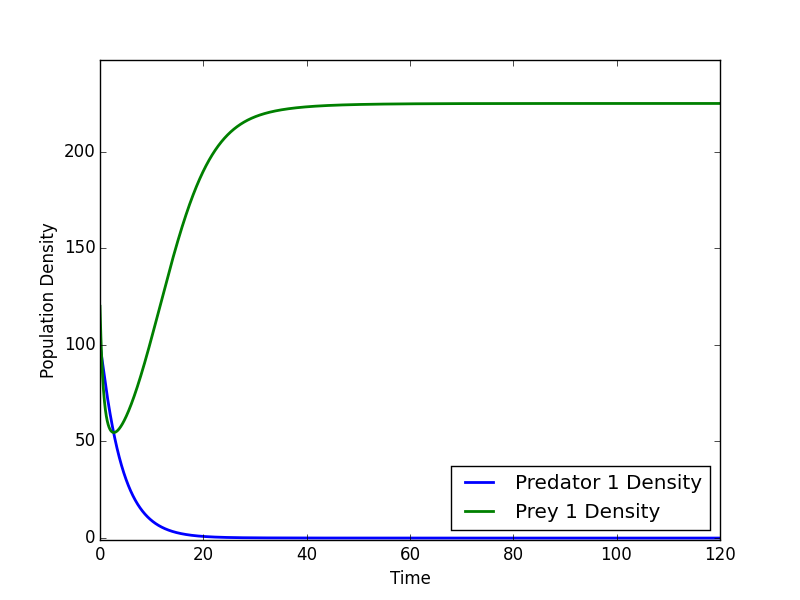
\includegraphics[width=9cm,height=6cm]{figures/1x1/constant_growth/densities_exclusion.png}
		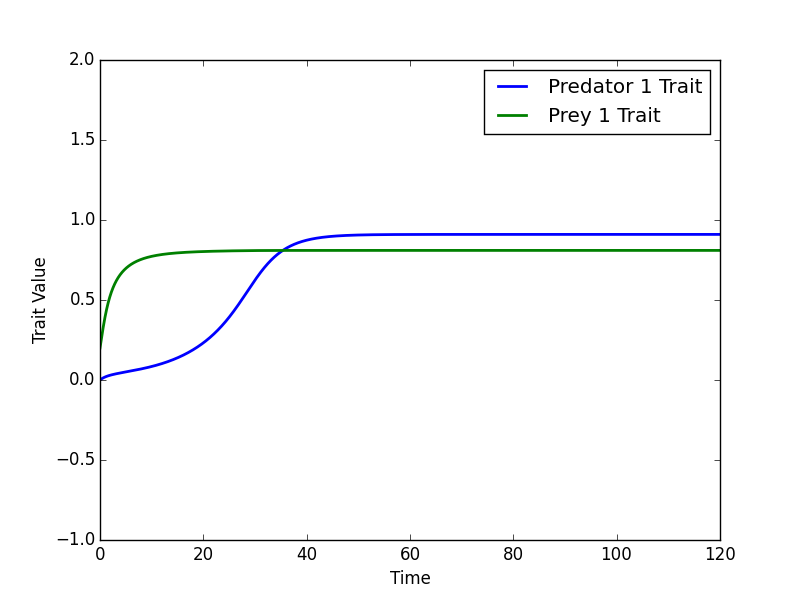
\includegraphics[width=9cm,height=6cm]{figures/1x1/constant_growth/traits_exclusion.png}
		\caption{Model 1: Exclusion Equilibrium}
		\label{fig:constant_growth_exclusion}
	\end{figure}
	\begin{figure}[h]
		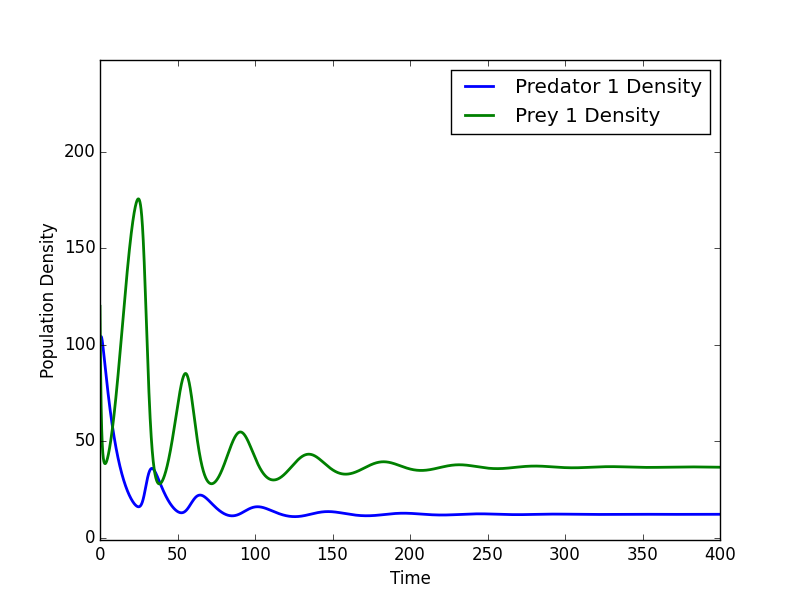
\includegraphics[width=9cm,height=6cm]{figures/1x1/constant_growth/densities_stable_coexistence.png}
		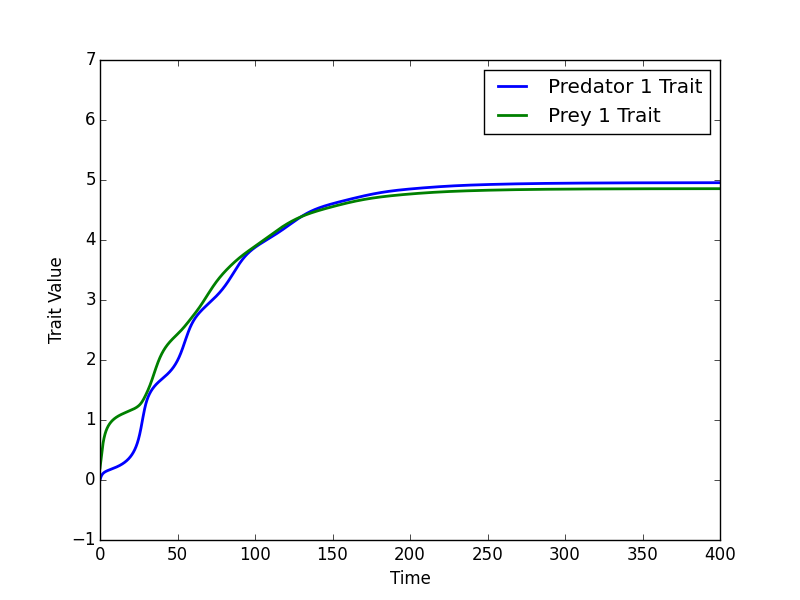
\includegraphics[width=9cm,height=6cm]{figures/1x1/constant_growth/traits_stable_coexistence.png}
		\caption{Model 1: Coexistence Equilibrium}
		\label{fig:constant_growth_coexistence_equilibrium}
	\end{figure}
	\begin{figure}[h]
		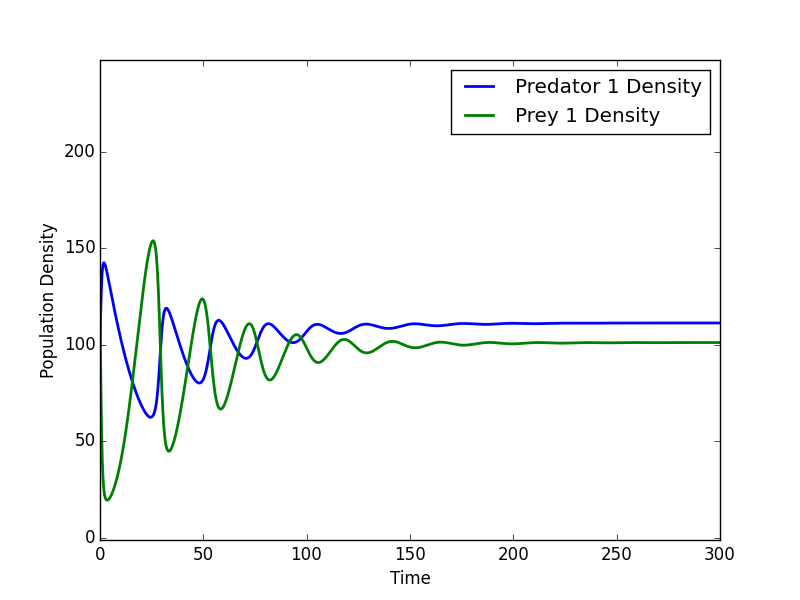
\includegraphics[width=9cm,height=6cm]{figures/1x1/constant_growth/densities_unstable_coexistence.png}
		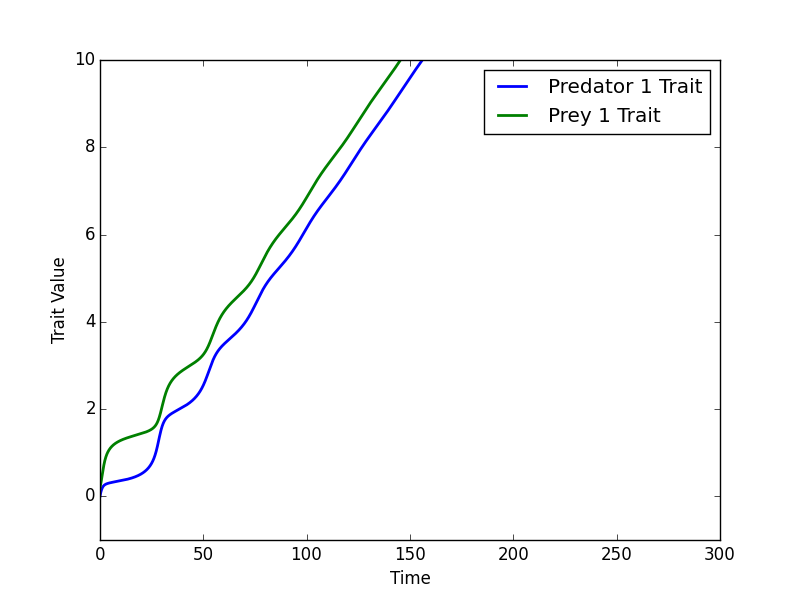
\includegraphics[width=9cm,height=6cm]{figures/1x1/constant_growth/traits_unstable_coexistence.png}
		\caption{Model 1: Non-Equilibrium Coexistence}
		\label{fig:constant_growth_non-equilibrium_coexistence}
	\end{figure}
	\begin{figure}[h]
		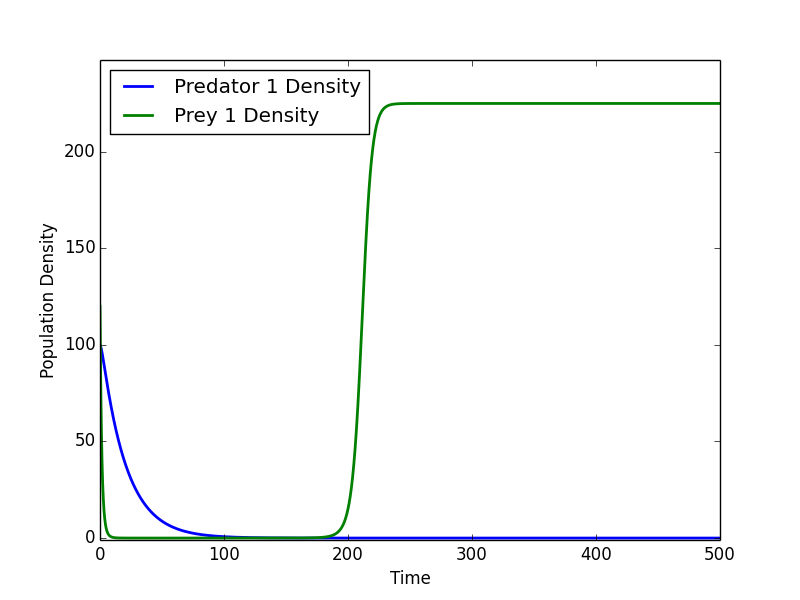
\includegraphics[width=9cm,height=6cm]{figures/1x1/variable_growth/stable_exclusion/densities.png}
		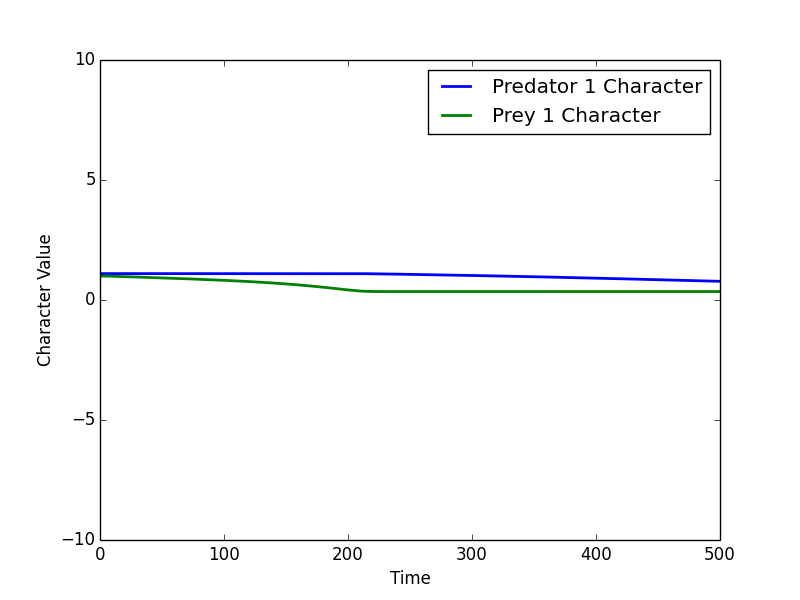
\includegraphics[width=9cm,height=6cm]{figures/1x1/variable_growth/stable_exclusion/traits.png}
		\caption{Model 2: Exclusion Equilibrium}
		\label{fig:variable_growth_exclusion}
	\end{figure}
	\begin{figure}[h]
		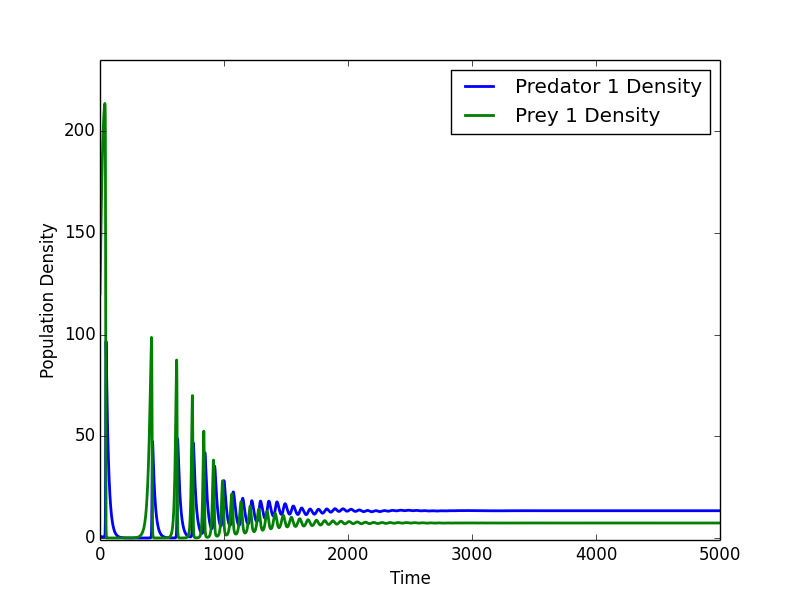
\includegraphics[width=9cm,height=6cm]{figures/1x1/variable_growth/stable_coexistence/densities.png}
		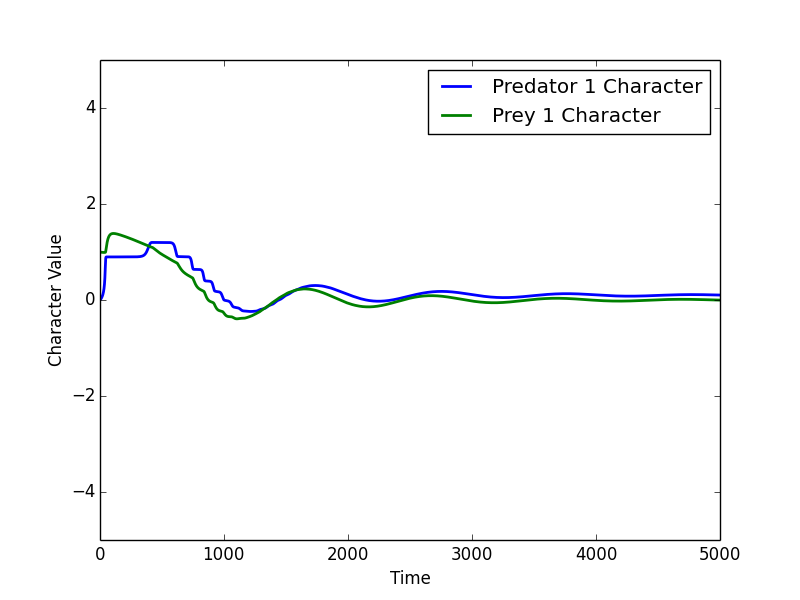
\includegraphics[width=9cm,height=6cm]{figures/1x1/variable_growth/stable_coexistence/traits.png}
		\caption{Model 2: Coexistence Equilibrium}
		\label{fig:variable_growth_coexistence_equilibrium}
	\end{figure}
	\begin{figure}[h]
		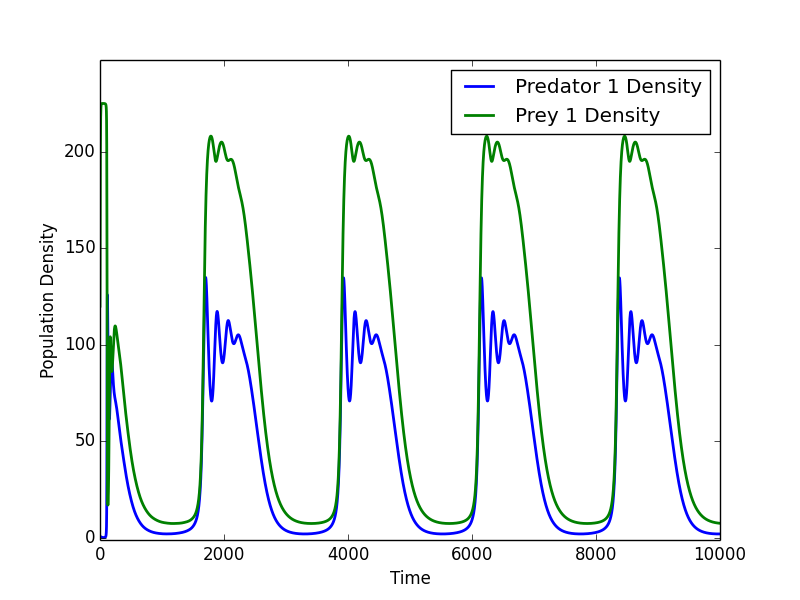
\includegraphics[width=9cm,height=6cm]{figures/1x1/variable_growth/stable_cycles/densities.png}
		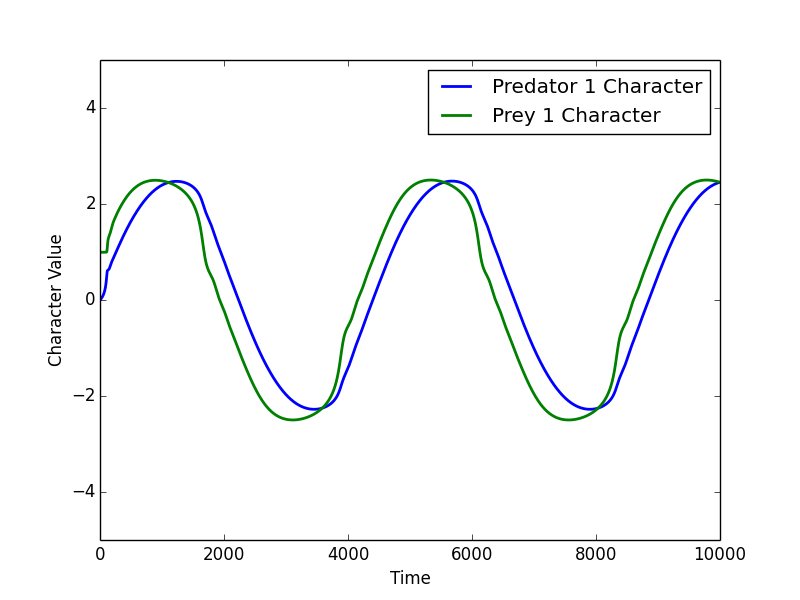
\includegraphics[width=9cm,height=6cm]{figures/1x1/variable_growth/stable_cycles/traits.png}
		\caption{Model 2: Non-Equilibrium, Cyclic Coexistence}
		\label{fig:variable_growth_stable_cycles}
	\end{figure}
\end{centering}
%% For two column figures and tables, use the following:

%% \begin{figure*}
%% \caption{Almost Sharp Front}\label{afoto}
%% \end{figure*}

%% \begin{table*}
%% \caption{Repeat length of longer allele by age of onset class}
%% \begin{tabular}{ccc}
%% table text
%% \end{tabular}
%% \end{table*}

%----------------------------------------------------------------------------------------

\end{document}